\textbf{Solve the boundary value problem $u_{xx}+4u_{x}+e^xu=\sin{(8x)}$ numerically on $[-1,1]$ with boundary conditions $u(\pm1)=0$. To 10 digits of accuracy, what is $u(0)$?}
\newline

We can express the BVP as
\begin{align*}
D^2u+4Du+\text{diag}(e^x)u &= f,\\
\left[D^2+4D+\text{diag}(e^x)\right]u &= f,\\
Mu &= f.
\end{align*}
where $D$ is the Chebyshev differentiation matrix and $f$ is the right hand side of the equation. Hence, we can calculate the solution to our BVP as
\begin{align*}
u &= M^{-1}f.
\end{align*}

The solution, using $N+1=51$ points (odd number of points to have a node exactly at $x=0$), is plotted in the figure 1. In the figure 2 we plot the value of $u(x=0)$ for different values of $N$. We see how with just $10+$ nodes we achieve high accuracy. The value of $u(x=0)$ obtained is
\begin{align*}
u(0) =  0.0095978572.
\end{align*}
The number of nodes needed to achieve 10 digits of accuracy was $N+1 = 23$.
\begin{figure}[H]
\centering
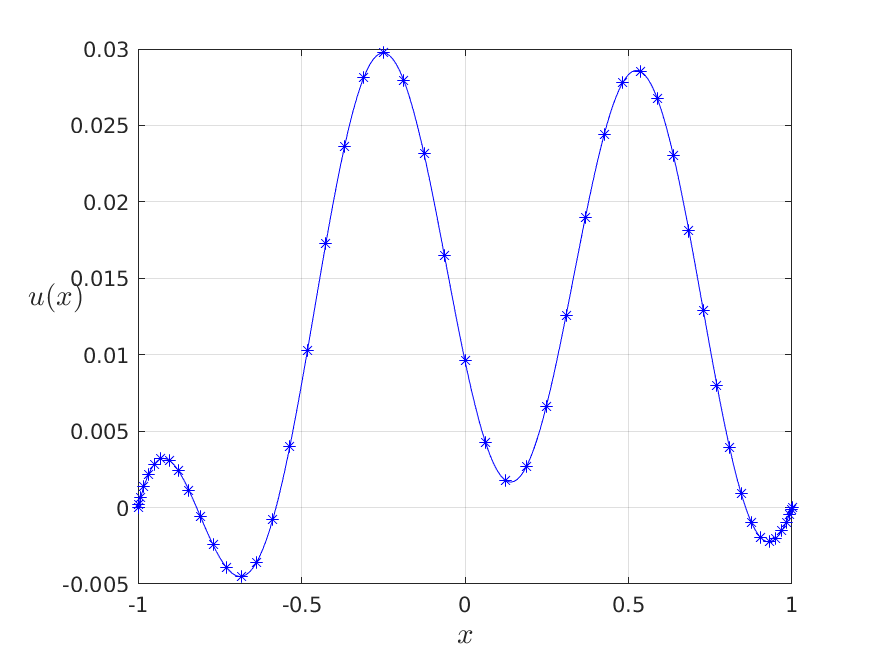
\includegraphics[scale=0.9]{P1_b.png}\caption{Solution to the BVP using Chebyshev matrices and 51 nodes.}
\end{figure}

\begin{figure}[H]
\centering
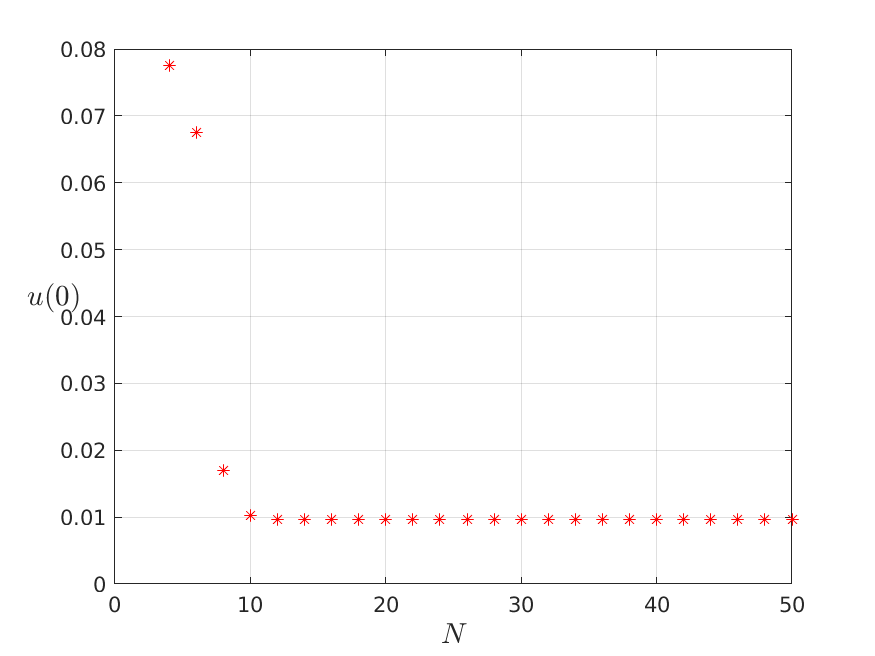
\includegraphics[scale=0.9]{P1_a.png}\caption{Value of $u(0)$ for different number of nodes.}
\end{figure}

\subsection*{Matlab code for this problem}

\begin{verbatim}
%% Homework 4, Problem 1 - Francisco Castillo
clear all; close all; clc;
labelfontsize = 14;

NN = 4:2:50;
for j=1:length(NN)
    N=NN(j);
    [D,x] = cheb(N); % D:(N+1)x(N+1), x:(N+1)x1
    D2 = D^2;
    D = D(2:N,2:N);
    D2 = D2(2:N,2:N);       % Zero Dirichlet BCs
    f = sin(8*x(2:N));
    E = diag(exp(x(2:N)));
    u = (D2+4*D+E)\f;
    u = [0;u;0];
    u0(j) = u(N/2+1);
end

figure
plot(NN,u0,'r*')
grid on
xlabel('$N$','fontsize',labelfontsize,'interpreter','latex')
ylabel('$u(0)$','fontsize',labelfontsize,'interpreter','latex')
set(get(gca,'ylabel'),'rotation',0)
txt = 'Latex/FIGURES/P1_a';
saveas(gcf,txt,'png')

xx = [x(end):.01:x(1)]';
uu = polyval(polyfit(x,u,N),xx);

figure
plot(x,u,'b*')
hold on
plot(xx,uu,'b')
grid on
xlabel('$x$','fontsize',labelfontsize,'interpreter','latex')
ylabel('$u(x)$','fontsize',labelfontsize,'interpreter','latex')
set(get(gca,'ylabel'),'rotation',0)
txt = 'Latex/FIGURES/P1_b';
saveas(gcf,txt,'png')
\end{verbatim}